%%%%%%%%%%%%%%%%%%%%%%%%%%%%%%%%%%%%%%%%%%%%%%%%%%%%%%%%%%%%%%%%%
\newpage
\section[Lineare Abbildungen (Wdh. Mathe 1)]{Lineare Abbildungen, Dualraum, Matrizen}
\Einleitung{Abschließend schauen wir uns einen Spezialfall von Abbildungen zwischen Vektorräumen an: Die linearen Abbildungen.\\
Was macht diese so besonders?\\
Sie haben die schöne Eigenschaft, dass sie sich (bei endlichdimensionalen VR) stets als Matrizen darstellen lassen. Wie genau diese aussehen, hängt von den Basen der beteiligten Vektorräume ab!\\
Mit Matrizen kann man angenehm rechnen und viele Eigenschaften der Abbildung schnell überblicken.}\\
\red{Anmerkung: Diese Notizen sind anders als das Skript strukturiert, da wir das für sinnvoller hielten.}
\subsection{Lineare Abbildungen: Von Vektorraum zu Vektorraum mit Stil}\label{ssec:LineareAbbildungen}
\begin{Def}
{Lineare Abbildungen}
Wir nennen eine \red{Abbildung} $F$ zwischen zwei Vektorräumen\footnote{beide über dem gleichen Körper $\mathbb{K}$} $V$ und $W$, also $F:V\to W$ \red{$\mathbb{K}$-linear}, wenn sie die folgenden Eigenschaften für alle $v,w\in V$ und $\lambda\in\mathbb{K}$ erfüllt:
\begin{align*}
    F(v+w)&=F(v)+F(w)\\
    F(\lambda v)&=\lambda F(v).
\end{align*}
\end{Def}
\begin{Def}
{Wiederholung: Raum der Abbildungen}
Wie letzte Woche schon gesehen, können wir alle möglichen Abbildungen $A$ zwischen zwei Mengen $X$ und $Y$, d. h. $A:X\to Y$, als Vektorraum auffassen.\footnote{Das bedeutetet, dass Linearkombinationen dieser Abbildungen wieder solche Abbildungen sind.} Diesen hatten wir als $\Abb(X,Y)$ definiert.
\end{Def}
\blue{Dieses Konzept ist auf den ersten Blick sehr seltsam: Wir fassen Abbildungen als Vektoren auf und können somit auch Linearkombinationen (z. B. $5A-3B:X\to Y$ mit $A,B\in\Abb(X,Y)$) bilden.}
\begin{Def}
{Raum der $\mathbb{K}$-linearen Abbildungen}
Sind $V$ und $W$ wieder Vektorräume über $\mathbb{K}$, so stellen wir fest, dass alle linearen Abbildungen von $V\to W$ einen Unterraum von $\Abb(V,W)$ bilden.\\
Diesen bezeichnen wir als \red{$\boxed{L(V,W)}$}.
\end{Def}
Anstatt eine lineare Abbildung über '$F:V\to W$ linear' zu definieren, können wir einfach $F\in L(V,W)$ schreiben.
\begin{figure}[htbp]
\centering
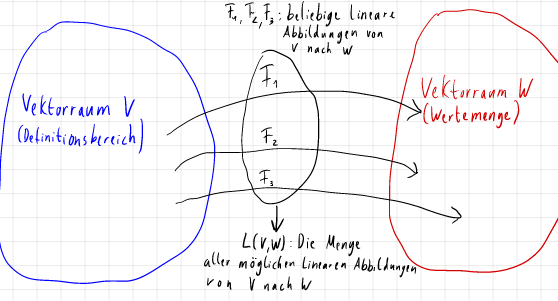
\includegraphics[width=.6\textwidth]{Dateien/00/12LinAbbSchaubild.PNG}
\caption*{Schaubild zu linearen Abbildungen. $\Abb(V,W)$ wäre hier noch eine größere Menge an Abbildungen als $L(V,W)$.}
\end{figure}
\begin{Beispiel}
{1D lineare Funktion (1/4)}
Für $V=\mathbb{R}$, $W=\mathbb{R}$ ist $F\in L(\mathbb{R},\mathbb{R}),\,F(x)=ax$ mit einer Konstante $a\in\mathbb{R}$ $\mathbb{R}$-linear, denn für alle $x,y\in V$, $\lambda\in\mathbb{R}$ gilt
\begin{align*}
    F(x+y)&=a(x+y)=ax+ay=F(x)+F(y)\\
    F(\lambda x)&=a\lambda x=\lambda ax=\lambda F(x).\, \checkmark
\end{align*}
\end{Beispiel}
\begin{Beispiel}
{Von 2D nach 1D (2/4)}
Für $V=\mathbb{R}^2$, $W=\mathbb{R}$ ist $F\in L(\mathbb{R}^2,\mathbb{R}),\,F\BracedIn{\Matrix{x\\y}}=F(x,y)=2x-7y$ $\mathbb{R}$-linear, denn für alle $v=\Matrix{x\\y},w=\Matrix{z\\a}\in \mathbb{R}^2$, $\lambda\in\mathbb{R}$ gilt
\begin{align*}
    F(v+w)&=F(x+z, y+a)=2(x+z)-7(y+a)=2x-7y+2z-7a=F(v)+F(w)\\
    F(\lambda v)&=F(\lambda x,\lambda y)=2\lambda x-7\lambda y y=\lambda(2x-7y)=\lambda F(v).\, \checkmark
\end{align*}
\end{Beispiel}
\begin{Beispiel}
{Quadratische Funktionen sind nicht linear (3/4)}
Die Abbildung $F\in\Abb(\mathbb{R},\mathbb{R}),\,F(x)=x^2$ ist nicht $\mathbb{R}$-linear, denn für $x=2\in\mathbb{R}$ gilt
\begin{align*}
    F(2+2)=4^2=16\neq 8=4+4=2^2+2^2=F(2)+F(2).\text{ \Lightning}
\end{align*}
\end{Beispiel}
\begin{Beispiel}
{Die Ableitung ist linear (4/4)}
Wie wir schon gesehen hatten, ist eine Eigenschaft der Ableitung\\
$A:C^1(\mathbb{R},\mathbb{R})\to C^0(\mathbb{R},\mathbb{R}),\, A(f)=f'$ die Linearität.\\
Da wir die stetig differenzierbaren Funktionen $C^1(\mathbb{R},\mathbb{R})$ und die stetigen Funktionen $C^0(\mathbb{R},\mathbb{R})$ als Vektorräume auffassen können, handelt es sich somit um eine lineare Abbildung.
\end{Beispiel}
Von nun an seien $U,V,W$ \underline{endlichdimensionale} Vektorräume über einem Körper $\mathbb{K}$. 
\begin{Satz}
{Satz}{Eindeutigkeit der Wirkung auf Basisvektoren}
Für $V,W$ mit $\dim V=n$ und mit einer festgelegten Basis $(b_1,b_2,...,b_n)$ von $V$ gibt es für jedes $n$-Tupel $(w_i)_{i=1,...,n}$ von Vektoren aus $W$ \underline{genau eine} lineare Abbildung mit $F(b_i)=w_i$.\\
Diese Abbildung ordnet also jedem Basisvektor aus $V$ einen der Vektoren aus dem Tupel zu und ist \underline{eindeutig}.
\end{Satz}
Dieser Satz ermöglicht später die Darstellung von $F$ über darstellende Matrizen bzgl. der Basen von $V$ und $W$ (siehe unten).
\begin{Satz}
{Satz}{Kompositionen linearer Abbildungen sind linear}
Seien $F\in L(U,V)$ und $G\in L(V,W)$.\\
Dann ist auch die Komposition $G\circ F:U\to W$ eine lineare Abbildung.
\end{Satz}
\begin{Satz}
{Satz}{Unterräume werden auf Unterräume abgebildet}
Sei $F\in L(V,W)$.\\
\begin{tabular}{c l}
\parbox[b]{8cm}{
Für jeden Unterraum $V'\subseteq V$ ist dessen Bild $F(V')\subseteq W$ ein Unterraum von $W$.\\
Zudem ist für jeden Unterraum $W'\subseteq W$ dessen Urbild $F^{-1}(W')\subseteq V$ ein Unterraum.\\
Im nebenstehenden Beispiel ist dies für eine Gerade, die ja ein Unterraum des $\mathbb{R}^2$ ist, veranschaulicht.
} & 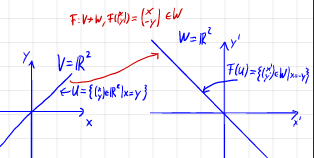
\includegraphics[width=.45\textwidth]{Dateien/00/12BeispielUnterraumUnterraum.PNG}
\end{tabular}
\end{Satz}
\subsubsection{Kern und Bild einer linearen Abbildung}\label{sssec:12KernBildDefinition}
Kennt ihr noch die grundlegenden Begriffe zu Abbildungen wie Injektivität und Surjektivität?\\
Diese werden nun wieder wichtig. Es stellt sich heraus, dass es aufgrund der Eigenschaften linearer Abbildungen ausreicht, zu schauen, ob nur der Nullvektor auf den Nullvektor abgebildet wird, um die Injektivität zu überprüfen.\\
So wie wir das Bild von allgemeinen Abbildungen kennengelernt hatten, interessiert uns nun das Bild von linearen Abbildungen. Stimmt die Dimension des Bildvektorraumes $F(V)$ mit der Dimension des Zielvektorraumes $W$ überein, so liegt Surjektivität vor. Diese Relationen greifen wir in Abschnitt \ref{ssec:Dimensionsformel} noch einmal auf, zunächst aber nur einige wichtige Definitionen:
\begin{Def}
{Kern von $F$}
Die Menge aller Vektoren aus $V$, die durch eine lineare Abbildung $F\in L(V,W)$ auf den \underline{Nullvektor} von $W$ abgebildet werden, nennen wir den \red{Kern von $F$}, geschrieben als\\
$\ker F= F^{-1}(\Vec{0})=\{v\in V\furdas F(v)=0\}\subseteq V$.
\end{Def}
\begin{Def}
{Bild von $F$}
Die Menge aller Vektoren aus $W$, die wir durch $F$ abbilden können, nennen wir das \red{Bild von F}, geschrieben als\\
$\im F=F(V)\subseteq W$.
\end{Def}
\blue{Aufgrund des vorhergehenden Satzes sind $\ker F\subseteq V$ und $\im F\subseteq W$ jeweils Unterräume von $V$ und $W$.}
\begin{figure}[htbp]
\centering
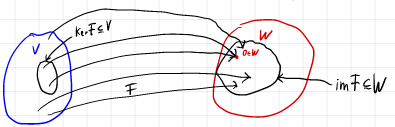
\includegraphics[width=.5\textwidth]{Dateien/00/12KernBild.PNG}
\caption*{Veranschaulichung von Kern und Bild}
\end{figure}
\subsection[Matrizen]{Matrizen\footnote{Laut \href{https://www.duden.de/rechtschreibung/Matrix}{Duden} ist die empfohlene Pluralschreibweise zwar Matrizes, aber irgendwie hört sich das komisch an - 'Matrizen' ist auch erlaubt.}}
Bevor wir tiefer in die linearen Abbildungen einsteigen, sollten wir uns mit ein paar zugrunde liegenden Definitionen vertraut machen.
\begin{Def}
{Matrix}
Wir definieren die Menge der \red{Matrizen} mit \red{$m$} Zeilen und \red{$n$} Spalten und Komponenten aus einem Körper $\mathbb{K}$ als
\begin{center}
    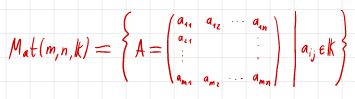
\includegraphics[width=.5\textwidth]{Dateien/00/12Matrixdefinition.PNG}
\end{center}
Mit der Notation $a_{ij}$ bezeichnen wir die insgesamt $m\cdot n$ Komponenten ($i=1,...,m$ und $j=1,...,n$).\\
Im Folgenden meint eine Einklammerung, dass alle Komponenten berücksichtigt werden, d. h. $(a_{ij}):=(a_{ij})_{i=1,...,m\, j=1,...,n}$.\\
Für $A=(a_{ij}), B=(b_{ij})\in\Met(m,n,\mathbb{K})$ und $\lambda\in\mathbb{K}$ bilden $(\Met(m,n,\mathbb{K}),+,\cdot, \mathbb{K})$ mit der Addition und der Multiplikation,
\begin{align*}
    +:&\quad(a_{ij})+(b_{ij})=(a_{ij}+b_{ij}),\\
    \cdot : & \quad\lambda (a_{ij})=(\lambda a_{ij})
\end{align*}
einen Vektorraum.
\end{Def}
\begin{Beispiel}
{Zeilenvektoren sind Matrizen (1/3)}
$A:=\Matrix{1 &2&3}\in\Met(1,3,\mathbb{R})$ ist eine $(1\times 3)$-Matrix.\\
Wir nennen $(1\times n)$-Matrizen auch \red{Zeilenvektoren}.
\end{Beispiel}
\begin{Beispiel}
{Spaltenvektoren sind Matrizen (2/3)}
$B:=\Matrix{-1\\0\\2}\in\Met(3,1,\mathbb{R})$ ist eine $(3\times 1)$-Matrix.\\
Wir nennen $(n\times 1)$-Matrizen auch \red{Spaltenvektoren}.
\end{Beispiel}
\begin{Beispiel}
{Linearkombination von Matrizen (3/3)}
$C:=\Matrix{1&3&4\\2&0&1}$ und $D:=\Matrix{-1&2&-2\\1.5&\pi &2}$ sind $(2\times 3)$-Matrizen. Es ist\\
\begin{equation*}
    -2C+D=\Matrix{-2&-6&-8\\-4&0&-2}+\Matrix{-1&2&-2\\1.5&\pi &2}=\Matrix{-3&-4&-10\\-2.5&\pi&0}.
\end{equation*}
\end{Beispiel}
\begin{Def}
{Matrixmultiplikation}
Seien $A=(a_{ij})\in\Met(m,n,\mathbb{K})$ und $B=(b_{ij})\in\Met(n,q,\mathbb{K})$.\\
Dann definieren wir als \red{Produkt} aus diesen Matrizen die Matrix
\begin{equation*}
    C=A\cdot B\in\Met(m,q,\mathbb{K}),\quad (c_{ik})=\sum_{j=1}^na_{ij}b_{jk}.
\end{equation*}
\end{Def}
\begin{Satz}
{Merksatz}{Mögliche Multiplikation}
Zum Testen, ob zwei Matrizen multiplizierbar sind, einfach die Dimensionen aufschreiben:
\begin{equation*}
    \boxed{m\times n\cdot p\times q}
\end{equation*}
ist nur möglich, wenn $n=p$.\\
Das Resultat ist eine $(m\times q)$-Matrix.
\end{Satz}
\begin{Beispiel}{Matrixmultiplikation}
Betrachte $C:=\Matrix{1&3&4\\2&0&1}$ und $D:=\Matrix{-1&2\\1&-1}.$\\
Welche Produkte sind möglich?
\begin{enumerate}
    \item $C\cdot D\rightarrow 2\times \overbrace{3\cdot 2}^{\neq} \times 2$. \Lightning
    \item $C^2\rightarrow 2\times \overbrace{3\cdot 2}^{\neq} \times 3$. \Lightning
    \item $D\cdot C\rightarrow 2\times \overbrace{2\cdot 2}^= \times 3\,\checkmark$ ($=2\times 3$). Hier ist
\begin{center}
    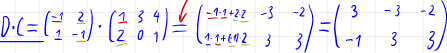
\includegraphics[width=.5\textwidth]{Dateien/00/12DMalC.PNG}
\end{center}
wobei ich (Fabian) mir den Schritt mit dem roten Pfeil immer so vorstelle, dass ich die einzelnen Spalten der hinteren Matrix auf die vordere draufklappe und damit die einzelnen Einträge bilde.
    \item $D^2\rightarrow 2\times \overbrace{2\cdot 2}^= \times 2\,\checkmark $ ($=2\times 2$). Hier haben wir
    \begin{equation*}
        D\cdot D=\Matrix{-1&2\\1&-1}\Matrix{-1&2\\1&-1}=\Matrix{1&-4\\-2&3}.
    \end{equation*}
\end{enumerate}
\end{Beispiel}
\begin{Def}
{Spur}
Für einige Anwendungen benötigt ihr später auch die \red{Spur}\footnote{engl. \textit{Trace}} von Matrizen.\\
Diese ist für quadratische Matrizen definiert und bezeichnet schlicht die Summe über alle Diagonalelemente:
\begin{equation*}
    \Tr:\Met(n,n,\mathbb{K})\to \mathbb{K},\quad A\mapsto \Tr(A)=\sum_{k=1}^na_{kk}.
\end{equation*}
\end{Def}
Die Spur findet vor allem in der Quantenmechanik Anwendung, wo mithilfe einer \textit{Dichtematrix} $\rho$ die Wahrscheinlichkeitsverteilung eines Systems widergespiegelt wird.\footnote{Siehe auch \href{https://de.wikipedia.org/wiki/Dichteoperator}{Wikipedia}.} Für die Normiertheit muss $\Tr(\rho)=1$ sein, die nicht-Diagonaleinträge symbolisieren die Übergangswahrscheinlichkeiten in andere Zustände.\\
Die Spur von $\rho^2$ gibt zudem Auskunft über die 'Reinheit' eines Systems.
\begin{Satz}
{Satz}{Vertauschbarkeit der Spur des Produktes}
Für $A\in\Met(m,n,\mathbb{K})$ und $B\in\Met(n,m,\mathbb{K})$ ist die Produktmatrix quadratisch.\\
Für deren Spur gilt
\begin{equation*}
    \Tr(\underbrace{A\cdot B}_{m\times m})=\Tr(\underbrace{B\cdot A}_{n\times n}).
\end{equation*}
Es lässt sich leicht zeigen, dass wir daher Matrizen innerhalb einer Spur zyklisch vertauschen können:\\
Für $A\in\Met(m,n,\mathbb{K})$, $B\in\Met(n,q,\mathbb{K})$ und $C\in\Met(q,m,\mathbb{K})$ gilt dann
\begin{equation*}
    \Tr(\underbrace{A\cdot B\cdot C}_{m\times m})=\Tr(\underbrace{C\cdot A\cdot B}_{q\times q})=\Tr(\underbrace{B\cdot C\cdot  A}_{n\times n}).
\end{equation*}
\end{Satz}


\subsubsection{Darstellende Matrizen: Lineare Abbildungen in Matrixdarstellung}
Nun erarbeiten wir uns die tolle Eigenschaft linearer Abbildungen, stets als Matrizen dargestellt werden zu können (zumindest, solange die beteiligten Vektorräume endlichdimensional sind).\\
Wie diese Matrizen aussehen, hängt aber von den Basen der Vektorräume ab! Daher wiederholen wir auch noch einmal den Basisbegriff.
\begin{Satz}
{Satz}{Kanonische Zuordnung}
Jeder linearen Abbildung $F\in L(\mathbb{K}^n,\mathbb{K}^m)$ können wir eine Matrix zuordnen, indem wir uns die \underline{Wirkung von $F$ auf die Basisvektoren} $(e_j)_{j=1,...,n}$ des $\mathbb{K}^n$ anschauen und diese als Matrix anordnen:
\begin{equation*}
    \varphi:L(\mathbb{K}^n,\mathbb{K}^m)\to \Met(m,n,\mathbb{K}),\, F\,\mapsto \varphi(F)=(F(e_1)\cdots F(e_n)).
\end{equation*}
\end{Satz}
\begin{Beispiel}{Kanonische Zuordnung}
Für $F:\mathbb{R}^2\to\mathbb{R}^3,\, F(x,y)=\Matrix{x+y\\2x-y\\5y}$ ist $F(e_1)=F(1,0)=\Matrix{1\\2\\0}$ und $F(e_2)=\Matrix{1\\-1\\5}$, wir haben also
\begin{equation*}
    \varphi(F)=\Matrix{1&1\\2&-1\\0&5}\in\Met(3,2,\mathbb{R}).
\end{equation*}
\end{Beispiel}
\begin{Def}
{Erinnerung: Basis}
Eine \red{Basis} eines Vektorraums $V$ der Dimension $\dim V= n$ ist eine linear unabhängige Familie von $n$ Vektoren, die den gesamten Vektorraum aufspannt,\footnote{alle Vektoren aus $V$ können also durch Linearkombination der Basisvektoren gebildet werden.} d. h. sie ist ein Erzeugendensystem von $V$.
\end{Def}
\begin{Beispiel}{Basen des $\mathbb{R}^3$}
Die Familien
\begin{align*}(e_1,e_2,e_3)&:=\BracedIn{\Matrix{1\\0\\0},\Matrix{0\\1\\0},\Matrix{0\\0\\1}},\\
(a_1,a_2,a_3)&:=\BracedIn{\Matrix{1\\1\\0},\Matrix{1\\0\\1},\Matrix{0\\-1\\-1}},\\
(b_1,b_2,b_3)&:=\BracedIn{\Matrix{1\\2\\3},\Matrix{4\\5\\6}\Matrix{7\\8\\-9}}
\end{align*}
sind jeweils Basen des $\mathbb{R}^3$.\\
Die Darstellung von Vektoren als Linearkombination hängt damit auch von der Basis ab:
\begin{equation*}
    v:=\Matrix{1\\1\\1}=e_1+e_2+e_3=\frac{1}{2}a_1+\frac{1}{2}a_2-\frac{1}{2}a_3=-\frac{1}{3}b_1+\frac{1}{3}b_2.
\end{equation*}
\end{Beispiel}
Wir haben gesehen, dass wir $F\in L(\mathbb{R}^n,\mathbb{R}^m)$ bzgl. der kanonischen Basis als Matrix darstellen können.\\
Dieses Konzept wollen wir nun auf lineare Abbildungen zwischen beliebigen (endlichdimensionalen) Vektorräumen $F\in L(V,W)$ mit beliebigen Basen von $V$ und $W$ erweitern.
\begin{Def}
{Darstellende Matrix}
Sei $B$ die Basis von $V$ (mit $\dim V=n$) und $B'$ die Basis von $W$ (mit $\dim W=m$).\\
Durch lineare Abbildungen $\phi_B:\mathbb{K}^n\to V,\,\phi_{B'}:\mathbb{K}^m\to W$, die so konstruiert sind, dass die kanonischen Einheitsvektoren des $\mathbb{K}^n$ bzw. $\mathbb{K}^m$ genau auf die Basen von $V$ und $W$ abgebildet werden, können wir $F$ durch den obigen Satz auf eine Matrix zurückführen:\\
Die \red{darstellende Matrix} $A\in\Met(m,n,\mathbb{K})$ bezüglich der Basen $B$ und $B'$ ist gegeben durch
\begin{equation*}
    Ae_j=(\phi^{-1}_{B'}\circ F\circ \phi_B)e_j
\end{equation*}
und wir schreiben $A=M_B^{B'}(F)$, um die verwendeten Basen zu verdeutlichen.\\
Für lineare Abbildungen $F\in L(\mathbb{K}^n,\mathbb{K}^m)$ nennen wir die darstellende Matrix bzgl. der Standardbasen die \red{kanonisch zugeordnete Matrix}.
\end{Def}
Das sieht auf den ersten Blick ziemlich kompliziert aus! Aber keine Angst, mit dem folgenden Satz kann man die darst. Matrix leicht finden, und es sollte auch noch klarer werden, wie man damit umgeht.
\begin{Satz}
{Satz}{Bestimmung der darstellenden Matrix}
Die darstellende Matrix $A=(a_{ij})=M_B^{B'}(F)$ einer linearen Abbildung $F\in L(V,W)$ ist durch folgende Gleichung bestimmt:
\begin{equation*}
    \boxed{F(b_{\red{k}})=\sum_{i=1}^ma_{i\red{k}}b'_i}.
\end{equation*}
Hierbei seien $b_k\in B$ Basisvektoren von $V$ und $b_i'\in B'$ die Basisvektoren von $W$.
\end{Satz}
\blue{Wir können also die darstellende Matrix einfach finden, indem wir uns die Wirkung von $F$ auf die Basisvektoren von $V$ anschauen und dann versuchen, die Matrixkomponenten als Koeffizienten der Linearkombinationen der Basisvektoren von $W$ zu finden.\footnote{Sorry für diesen Schachtelsatz, nach ein paar mal lesen oder vielleicht nach Betrachtung der Beispiele sollte er Sinn ergeben.}\\
\textbf{Anmerkung}: Für die Beispiele haben wir den eher anwendungsbezogenen zweiten Weg genommen. Falls euch interessiert, wie genau das mit den Abbildung $\phi_B$ und $\phi_{B'}$ aussehen würde, könnt ihr das in Abschnitt \ref{sssec:12DarstMatrixlang} nachlesen.}
\begin{Beispiel}
{Lineare Abbildung im $\mathbb{R}^2$ (1/2)}
\begin{tabular}{c l}
\parbox[b]{9cm}{
Wir betrachten $V=\mathbb{R}^2$, $W=\mathbb{R}^2$ und definieren die Basen
\begin{align*}
    B_V:&=(b_1,b_2)=\BracedIn{\Matrix{1\\1},\Matrix{-1\\1}},\\ B_W':&=(b_1',b_2')=\BracedIn{\Matrix{1\\3},\Matrix{2\\0}}.
\end{align*}
} & 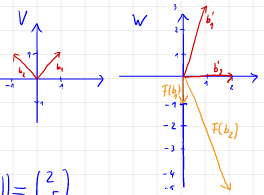
\includegraphics[width=.3\textwidth]{Dateien/00/12BeispielEbeneLinAbb.PNG}
\end{tabular}\\
Zudem sei unsere lineare Abbildung $F:V\to W$ durch
\begin{equation*}
    F(x,y)=\Matrix{y-x\\2x-3y}
\end{equation*}
definiert. 
\begin{itemize}
    \item Was macht $F$ mit den Basisvektoren von $V$?
    \begin{equation*}
        F(b_1)=F(1,1)=\Matrix{0\\-1},\quad F(b_2)=F(-1,1)=\Matrix{2\\-5}.
    \end{equation*}
    Um die darstellende Matrix bzgl. $B$ und $B'$ zu finden, müssen wir gucken, wie sich $F(b_1)$ und $F(b_2)$ durch $b_1'$ und $b_2'$ ausdrücken lassen.
    \item $F(b_1)$ und $F(b_2)$ als Linearkombination von $b_1'$ und $b_2'$:
    \begin{align*}
        \lambda_1b_1'+\lambda_2b_2'=F(b_1)&\Rightarrow \Matrix{1&2\\3&0}\Matrix{\lambda_1\\\lambda_2}=\Matrix{0\\-1}\rightarrow\lambda_1=-\frac{1}{3}\rightarrow\lambda_2=\frac{1}{6}\\
        \lambda_3b_1'+\lambda_4b_2'=F(b_1)&\Rightarrow \Matrix{1&2\\3&0}\Matrix{\lambda_3\\\lambda_4}=\Matrix{2\\-5}\rightarrow\lambda_3=-\frac{5}{3}\rightarrow\lambda_4=\frac{11}{6}
    \end{align*}
    Wir finden also:
    \begin{equation*}
        F(b_1)=-\frac{1}{3}b_1'+\frac{1}{6}b_2',\quad F(b_2)=-\frac{5}{3}b_1'+\frac{11}{6}b_2'.
    \end{equation*}
    \item Darstellende Matrix ablesen:\\
    Damit haben wir die Komponenten der darstellenden Matrix schon gefunden, denn es gilt ja 
\begin{equation*}
    \boxed{F(b_{\red{k}})=\sum_{i=1}^ma_{i\red{k}}b'_i}.
\end{equation*}
    Somit ist z. B. $F(b_1)=a_{11} b_1'+a_{21}b_2'$, also
    \begin{equation*}
        M_B^{B'}(F)=\Matrix{a_{11}&a_{12}\\a_{21}&a_{22}}=\Matrix{-1/3&-5/3\\1/6&11/6}=\frac{1}{6}\Matrix{-2&10\\1&11}.
    \end{equation*}
\end{itemize}
Und warum jetzt der ganze Aufwand?\\
Wir können jetzt beliebige Vektoren aus $V$, die wir bzgl. der Basis $B$ dargestellt haben, auf Vektoren bzgl. der Basis $B'$ aus $W$ abbilden!\\
Sei z. B. $v=\Matrix{3\\6}\in V$ bzgl. der Basis $B$,\footnote{Achtung, bzgl. der kanonischen Basis (wie ihr es vielleicht intuitiv kennt) sieht dieser Vektor anders aus!} d. h. $v=3b_1+6b_2$.\\
Dieser wird auf
\begin{equation*}
    w=M_B^{B'}(F)\cdot v=\frac{1}{6}\Matrix{-2&10\\1&11}\Matrix{3\\6}=\frac{1}{6}\Matrix{-6-60\\3+66}=\Matrix{-11\\23/2}
\end{equation*}
bzgl. der Basis $B'$, d. h. $w=-11b_1'+\frac{23}{2}b_2'$ abgebildet.
\begin{center}
    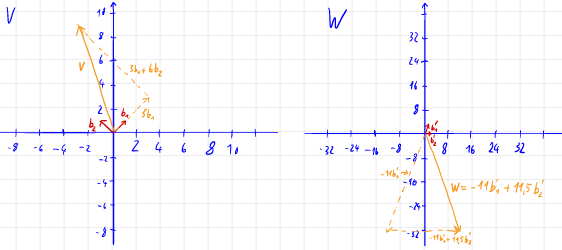
\includegraphics[width=.7\textwidth]{Dateien/00/12BeispielEbeneLinAbbB.PNG}
\end{center}
\textbf{Vergleich}:\\
Andererseits können wir $v$ und $w$ auch bzgl. der Standardbasen schreiben, denn dann sind
\begin{equation*}
    v=3b_1+6b_2=\Matrix{3-6\\3+6}=\Matrix{-3\\9},\quad w=-11b_1'+\frac{23}{2}b_2'=\Matrix{-11+23\\-33}=\Matrix{12\\-33}.
\end{equation*}
Wie sieht $F$ bzgl. der Standardbasen aus?\\ $F(e_1)=\Matrix{-1\\2}=-e_1'+2e_2'$ und $F(e_2)=\Matrix{1\\-3}=e_1'-3e_2'$.\\
Hier können wir die darstellende Matrix einfach ablesen, da die resultierenden Vektoren ja schon Linearkombinationen der kanonischen Einheitsvektoren von $W$ sind.
\begin{equation*}
    M_E^{E'}(F)=\Matrix{-1&1\\2 &-3}.
\end{equation*}
Und tatsächlich sehen wir:
\begin{equation*}
    F(v)=\Matrix{-1&1\\2 &-3}\Matrix{-3\\9}=\Matrix{12\\-33}=w.\,\checkmark
\end{equation*}
(Dafür bräuchten wir $M_E^{E'}$ eigentlich nicht, wir hätten auch $v$ einfach in $F$ einsetzen können.)
\end{Beispiel}
\begin{Beispiel}
{Der Link zum Vektorraum der Polynome (2/2)}\label{beisp:12DarstMatrix}
Sei $V=\mathbb{R}^2$ mit der Basis 
\begin{align*}
    B_V:&=(b_1,b_2)=\BracedIn{\Matrix{1\\1},\Matrix{-1\\1}}
\end{align*}
wie im vorherigen Beispiel.\\
Sei $W=\mathbb{R}[x]_{\leq 2}$ der 3-dimensionale Vektorraum der Polynome mit Grad $\leq2$ mit der Basis
\begin{equation*}
    B'=(b_1',b_2',b_3')=\BracedIn{(1+2x),(3x^2),(-x)}.
\end{equation*}
Sei unsere lineare Abbildung nun definiert als
\begin{equation*}
    F:\mathbb{R}^2\to \mathbb{R}[x]_{\leq 2},\,F(a,b)=a+(a-b)x+5bx^2\quad (\text{z. B. } F(1,2)=1-x+10x^2).
\end{equation*}
Wir notieren schonmal, dass diese Abbildung bzgl. der kanonischen Basen $E=(e_1,e_2)$ und $E'=(e_1',e_2',e_3')=((1),(x),(x^2))$ so aussieht:
\begin{equation*}
    M_E^{E'}(F)=\Matrix{1&0\\1&-1\\0&5}.
\end{equation*}
\begin{itemize}
    \item Was macht $F$ mit den Basisvektoren von $V$?
    \begin{eqnarray*}
        F(b_1)&=&F(1,1)\overset{\footnote{Einsetzungsweg}}{=}1+0x+5x^2=1+5x^2,\\
        F(b_2)&=&F(-1,1)\overset{\footnote{Bei gegebener darst. Matrix bzgl. der kanonischen Basen ist auch der Matrixmultiplikationsweg möglich.}}{=}\Matrix{1&0\\1&-1\\0&5}\Matrix{-1\\1}=\Matrix{-1\\-2\\5}=-1-2x+5x^2
    \end{eqnarray*}
    \item $F(b_1)$ und $F(b_2)$ als Linearkombination von $b_1'$, $b_2'$ und $b_3'$:\\
    Wir haben die Gleichungen
    \begin{equation*}
        \lambda_1b_1'+\lambda_2b_2'+\lambda_3b_3'=1+5x^2,\quad \lambda_4b_1'+\lambda_5b_2'+\lambda_6b_3'=-1-2x+5x^2,
    \end{equation*}
    die wir mit dem Gaußalgorithmus lösen können:
\begin{center}
    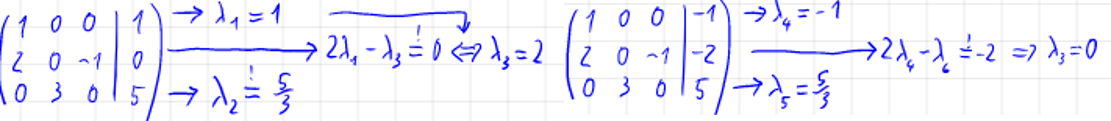
\includegraphics[width=.7\textwidth]{Dateien/00/12LsgGleichungssystem.png}
\end{center}
    \item Wir sehen also, dass
    \begin{equation*}
        1b_1'+\frac{5}{3}b_2'+2b_3'=1+5x^2,\quad -1b_1'+\frac{5}{3}b_2'+0b_3'=-1-2x+5x^2,
    \end{equation*}
    sodass wir die Koeffizienten für die darstellende Matrix nur noch ablesen brauchen:
    \begin{equation*}
        M_B^{B'}(F)=\Matrix{a_{11}&a_{12}\\a_{21}&a_{22}\\a_{31}&a_{32}}=\Matrix{1&-1\\5/3&5/3\\2&0}.
    \end{equation*}
    \item Anwendung:\\
    Wenn wir uns z. B. fragen, auf welchen Vektor $\in W$ der Vektor $v=2b_1-3b_2\in V$ abgebildet wird, reicht es, diesen mit $M_B^{B'}$ zu multiplizieren:
    \begin{align*}
        F(v)&=M_B^{B'}(F)\cdot v=\Matrix{1&-1\\5/3&5/3\\2&0}\Matrix{2\\-3}=\Matrix{5\\-5/3\\4}\\
        \Rightarrow w&=5b_1'-\frac{5}{3}b_2'+4b_3'=f(1+x)-\frac{5}{3}3x^2+4(-x)=5+6x-5x^2.
    \end{align*}
    Der Vergleich mit direktem Einsetzen liefert:
    \begin{equation*}
        F(v)=F\BracedIn{2\Matrix{1\\1}-3\Matrix{-1\\1}}=F(5,-1)=5+6x-5x^2.\,\checkmark
    \end{equation*}
\end{itemize}
\end{Beispiel}
\begin{Satz}
{Satz}{Verknüpfung linearer Abbildungen}
Seien $V,V',V''$ jeweils endlichdimensionale\footnote{da wir sonst ja keine darstellenden Matrizen definiert haben} Vektorräume mit den Basen $B,B',B''$. Seien $F\in L(V,V')$ und $G\in L(V',V'')$ lineare Abbildungen zwischen diesen Vektorräumen.\\
Dann ist $G\circ F\in L(V,V'')$ und für die darstellenden Matrizen gilt
\begin{equation*}
    M_B^{B''}(G\circ F)=M_{B'}^{B''}(G)M_B^{B'}(F).
\end{equation*}
\blue{Die darstellende Matrix einer verknüpften linearen Abbildung ist einfach das Produkt aus den darstellenden Matrizen der beteiligten Abbildungen.}
\end{Satz}
\begin{Beispiel}{Anwendung der Verknüpfung}\label{beisp:12VerknupfungLinAbb}
Seien $F:\mathbb{R}^3\to\mathbb{R},\,F(x,y,z)=3x+y-z$ und $G:\mathbb{R}\to \mathbb{R}^2,\,G(x)=\Matrix{2x\\-5x}$ lineare Abbildungen zwischen den Vektorräumen $\mathbb{R}^3,\mathbb{R},\mathbb{R}^2$ (mit den Basen $B,B',B''$).\\
Dann haben wir
\begin{equation*}
    (G\circ F):\mathbb{R}^3\to\mathbb{R}^2,\, (G\circ F)(x,y,z)=G(3x+y-z)=\Matrix{6x+2y-2z\\-15x-5y+5z}.
\end{equation*}
Seien $B,B',B''$ nun die Standardbasen von $\mathbb{R}^3,\mathbb{R},\mathbb{R}^2$. Dann ist
\begin{equation*}
    M_B^{B'}(F)=\Matrix{3 & 1 &-1},\quad M_{B'}^{B''}(G)=\Matrix{2\\-5}.
\end{equation*}
Deren Verknüpfung stimmt mit dem überein, was wir erwarten würden:
\begin{equation*}
    M_B^{B''}(G\circ F)=M_{B'}^{B''}(G)M_{B}^{B'}(F)=\Matrix{2\\-5}\cdot \Matrix{3&1&-1}=\Matrix{6&2&-2\\-15&-5&5}.\,\checkmark
\end{equation*}
\end{Beispiel}
\subsection{Zusammenhänge zwischen Rang, Dimension und Bijektivität}
Nun lernen wir eine wichtige Klassifikation von linearen Abbildungen kennen: Den sog. \textit{Rang}, der Auskunft über enorm viel gibt.\\
Wie sich herausstellen wird, können wir den bei Abbildungen zwischen endlichdimensionalen Vektorräumen einfach an der darstellenden Matrix ablesen, wenn wir diese auf Zeilenstufenform bringen. Auf geht's!\\
$V$ und $W$ seien im Folgenden weiterhin endlichdimensionale Vektorräume über $\mathbb{K}$.
\begin{Def}
{Rang einer Matrix}
Der \red{Rang} einer Matrix entspricht der \underline{Anzahl an linear unabhängigen Spalten} (bzw. Zeilen) der Matrix.\\
Also ist der Rang die Anzahl der Zeilen, die nach Anwendung des Gauß-Algorithmus nicht 0 werden.
\end{Def}
\begin{Def}
{Rang einer Abbildung}
Wir ordnen jeder linearen Abbildung $F:V\to W$ die \underline{positive}\footnote{inklusive 0} ganze Zahl
\begin{equation}
    \boxed{\rg F=\dim(\im F)}
\end{equation}
zu und nennen diese den \red{Rang von $F$}.\\
Der Rang entspricht also der Dimension des Bildes, und wir sehen schon, dass wir damit vielleicht einen Zusammenhang zur Surjektivität hergestellt haben.
\end{Def}
\begin{Satz}
{Satz}{Satz über den Rang}
Über die darstellende Matrix bzgl. beliebiger Basen $B,B'$ von $V$ und $W$ können wir diesen Rang bestimmen, denn es gilt
\begin{equation*}
    \rg F=\rg (M_B^{B'}(F)).
\end{equation*}
\blue{Interessanterweise hängt also das Aussehen der darst. Matrix von den Basen ab, der Rang ist aber invariant.}
\end{Satz}
\begin{Def}
{Transponieren einer Matrix}
Wir nennen eine an der Mitteldiagonalen gespiegelte Matrix $A^T$ die zu $A$ \red{transponierte} Matrix ($(a_{ij})^T=(a_{ji})$).\\
Das sieht dann z. B. so aus:
\begin{equation*}
    \Matrix{a&b\\c&d\\e&f}^T=\Matrix{a&c&e\\b&d&f}.
\end{equation*}
\end{Def}
\begin{Satz}
{Satz}{Zeilenrang {=} Spaltenrang}
Um den Rang einer Maxtrix zu bestimmen, ist es egal, ob wir diese \underline{transponieren}, bevor wir den Gauß-Algorithmus anwenden.
\end{Satz}
\begin{Beispiel}{Matrix mit vollem Rang (1/4)}
Die folgende Matrix hat $\rg A=3$:
\begin{equation*}
    A=\Matrix{1&0&0\\0&1&0\\0&0&1}.
\end{equation*}
\blue{Wenn keine Nullspalten/Zeilen auftreten, sagt man auch, die Matrix habe \red{vollen Rang}.}
\end{Beispiel}
\begin{Beispiel}{Matrix und Transponierte (2/4)}
Die folgende Matrix hat $\rg B= 2$, denn über den Gaußalgorithmus können wir sie umformen:
\begin{equation*}
    B=\Matrix{1&0&0\\0&1&1\\5&-5&-5}\overset{\text{Gauß}}{\rightarrow}\Matrix{1&0&0\\0&1&1\\0&0&0}.
\end{equation*}
Andererseits könnten wir auch
\begin{equation*}
    B^T=\Matrix{1&0&5\\0&1&-5\\0&1&-5}
\end{equation*}
betrachten, welche ebenfalls $\rg B^T=2$ hat.
\end{Beispiel}
\begin{Beispiel}
{Man sieht ihr den maximalen Rang an (3/4)}
Die folgende Matrix kann aufgrund des Satzes über das Transponieren maximal $\rg C\leq 2$ haben:
\begin{equation*}
    C=\Matrix{1&2\\3&4\\5&6}.
\end{equation*}
Betrachten wir $C^T$, so sehen wir:
\begin{equation*}
    C^T=\Matrix{1&3&5\\2&4&6}\overset{(II)-2(I)}{\to}\Matrix{1&3&5\\0&-2&-4}\Rightarrow\rg C^T=\rg C=2.
\end{equation*}
\end{Beispiel}
\begin{Beispiel}
{Rang einer verknüpften linearen Abbildung (4/4)}
Wir gucken uns wieder\\
$F:\mathbb{R}^3\to\mathbb{R},\,F(x,y,z)=3x+y-z$ und $G:\mathbb{R}\to \mathbb{R}^2,\,G(x)=\Matrix{2x\\-5x}$\\
(aus \hyperref[beisp:12VerknupfungLinAbb]{Bsp. 13.13}) an.\\
Da die Wahl der Basen für den Rang egal ist, wählen wir wieder die kanonischen Basen und haben
\begin{align*}
    \rg F&=\rg (M_B^{B'}(F))=\rg\Matrix{3&1&-1}=1\\
    \rg G &=\rg (M_{B'}^{B''}(G))=\rg \Matrix{2\\-5}=1\\
    \rg (G\circ F)&=\rg \Matrix{6&2&-2\\-15&-5 &5}\overset{(I)/2, (II)/5}{=}\rg \Matrix{3&1&-1\\-3&-1&1}\overset{(II)-(I)}{=}\rg\Matrix{3&1&-1\\0&0&0}=1.
\end{align*}
\end{Beispiel}
\subsubsection{Die Dimensionsformel und ihre Folgen}\label{ssec:Dimensionsformel}
\begin{Satz}
{Satz}{Dimensionsformel}
Für Vektorräume $V,W$ mit $\dim V=n\leq \infty$ und eine lineare Abbildung $F\in L(V,W)$ gilt:
\begin{equation*}
    \boxed{\rg F+\dim \ker F=\dim V}.
\end{equation*}
Die Dimension des Urbildraumes entspricht also der Summe aus der Dimension des Bildraumes und der Dimension des Raumes aller Vektoren aus $V$, die auf den Nullvektor abgebildet werden (vergl. Abschnitt \ref{sssec:12KernBildDefinition}).
\end{Satz}
\begin{Satz}
{Merksatz}{Surjektivität linearer Abbildungen}
Wie schon bei allgemeinen Abbildungen zwischen beliebigen Mengen nennen wir\\ $F\in L(V,W)$ \red{surjektiv}, wenn der gesamte Wertebereich getroffen wird, d. h. $F(V)=\im F\overset{!}{=}W$.\\
Aufgrund der Definition von $\rg F=\dim \im F$ gilt:
\begin{equation*}
    F\text{ surjektiv }\Leftrightarrow \rg F=\dim W.
\end{equation*}
\end{Satz}
\blue{Daraus folgen ein paar interessante Erkenntnisse:\\
$F$ kann nur surjektiv sein, wenn $\boxed{\dim V\geq \dim W}$.\\
Zudem ist das \underline{Bild der Basisvektoren} $(F(b_i))_i$ mit $(b_i)_i$ einer Basis von $V$ ein \underline{Erzeugendensystem} von $W$, wenn $F$ surjektiv ist.}
\begin{Satz}
{Merksatz}{Injektivität linearer Abbildungen}
Falls \underline{nur} der Nullvektor von $V$ durch $F\in L(V,W)$ auf den Nullvektor von $W$ abgebildet wird, d. h. $\ker F=\{\Vec{0}\}\subseteq V$, so ist $F$ \red{injektiv} (und umgekehrt).\\
Aufgrund der Dimensionsformel gilt dann (mit $\dim\ker F=0$)
\begin{equation*}
    F\text{ injektiv }\Leftrightarrow \rg F=\dim V.
\end{equation*}
\end{Satz}
\blue{Hier sehen wir nun:\\
$F$ kann nur injektiv sein, wenn $\boxed{\dim V\leq \dim W}$.\\
Zudem ist das \underline{Bild der Basisvektoren} $(F(b_i))_i$ \underline{linear unabhängig} in $W$, wenn $F$ injektiv ist.}
\subsubsection{Isomorphismen}\label{sssec:Isomorphismen}
Wir haben also nun schon einige Erkenntnisse zusammengetragen. Sicher könnt ihr nun 12 und 13 zusammenzählen und euch ausmalen, was besonderes passiert, wenn $\dim V=\dim W$ ist und sowohl Surjektivität als auch Injektivität von $F$ gegeben sind.
\begin{Def}
{Isomorphismus}
Wir nennen $F\in L(V,W)$ einen \red{Isomorphismus}, wenn $F$ \underline{injektiv und surjektiv} ist, d. h. $\ker F=\{0\}$ und $\im F=W$.\\
Für endlichdimensionale Vektorräume $V$ und $W$ gilt dann
\begin{equation*}
    F\text{ ist Isomorphismus }\Leftrightarrow \rg F\overset{\footnote{Dimensionsformel mit $\dim\ker F=0$}}{=}\dim V=\dim W.
\end{equation*}
\end{Def}
\blue{Zudem bildet das Bild der Basisvektoren $(F(b_i)_i)$ eine Basis\footnote{denn wie wir gesehen hatten sind diese Vektoren linear unabhängig aufgrund der Injektivität, und ein Erzeugendensystem aufgrund der Surjektivität.} von $W$, wenn $F$ bijektiv ist.}
\begin{Def}
{Isomorphie}
Wir nennen zwei Vektorräume $V$ und $W$ \red{isomorph}, wenn es einen Isomorphismmus von Vektorräumen gibt, d. h. wenn eine \underline{bijektive} lineare Abbildung $F:V\to W$ existiert.\\
\blue{Endlichdimensionale Vektorräume sind genau dann isomorph, wenn $\boxed{\dim V=\dim W}$.}
\end{Def}
\begin{Satz}
{Satz}{Linearität der Umkehrabbildung}
Ist $F:V\to W$ ein Isomorphismus, so ist die Umkehrabbildung $F^{-1}:W\to V$ ebenfalls linear.
\end{Satz}
\begin{Beispiel}
{Die Identitätsabbildung (1/4)}
Die (lineare) Identitätsabbildung $\Id: \mathbb{R}^n\to\mathbb{R}^n,\, \Id(x)=x$ ist ein Isomorphismus, denn die darstellende Matrix bzgl. der Standardbasen ist die $n\times n$-Einheitsmatrix
\begin{center}
    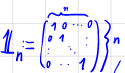
\includegraphics[width=.2\textwidth]{Dateien/00/12Einheitsmatrix.PNG}
\end{center}
weshalb $\rg F=\rg \mathds{1}_n=n=\dim\mathbb{R}^n=\dim\mathbb{R}^n$.
\end{Beispiel}
\begin{Beispiel}
{Verknüpfte Abbildung überprüfen (2/4)}
Wir gucken uns wieder\\
$F:\mathbb{R}^3\to\mathbb{R},\,F(x,y,z)=3x+y-z$ und $G:\mathbb{R}\to \mathbb{R}^2,\,G(x)=\Matrix{2x\\-5x}$\\
(aus \hyperref[beisp:12VerknupfungLinAbb]{Bsp. 13.13}) an.\\
Zunächst stellen wir fest, dass $F$ nicht injektiv sein kann, da $\dim \mathbb{R}^3>1=\dim \mathbb{R}$.\\
$G$ kann hingegen nicht surjektiv sein, da $\dim \mathbb{R}=1<2=\dim\mathbb{R}^2$.\\
Wir hatten gesehen, dass $\rg F=1$. Somit ist $F$ surjektiv.\\
Die Dimension des Kerns ist also nach der Dimensionsformel\\
$\dim\ker F=\dim \mathbb{R}^3-\rg F=2$.\\
\blue{Da der Kern ein Unterraum von $V$ ist, können wir dort auch eine Basis bestimmen. Dies schauen wir uns im nächsten Beispiel an.}\\
Es ist zudem $\rg G=1$. Somit ist $G$ injektiv (der Bildraum hat also ebenfalls eine Dimension von 1).\\
Die Verkettung $G\circ F:\mathbb{R}^3\to \mathbb{R}^2$ ist weder injektiv noch surjektiv, da\\
$\dim\mathbb{R}^3=3\neq1=\rg(G\circ F)$ (\Lightning Injektivität) und\\ $\dim \mathbb{R}^2=2\neq 1=\rg(G\circ F)$ (\Lightning Surjektivität).
\end{Beispiel}
\begin{Beispiel}
{Basis des Kerns bestimmen (3/4)}
Wir bestimmen jetzt eine Basis des Kerns von $F:\mathbb{R}^3\to\mathbb{R},\,F(x,y,z)=3x+y-z$, also dem Unterraum von $\mathbb{R}^3$, der von $F$ auf den Nullvektor abgebildet wird:
\begin{enumerate}
    \item \textbf{Gleichung aufstellen}:
    \begin{equation*}
        F(v)=\Vec{0}\overset{\footnote{Darst. Matrix bzgl. der Standardbasis}}{\to} \Matrix{3&1&-1}\Matrix{a\\b\\c}=0 \Leftrightarrow 3a+b-c=0.
    \end{equation*}
    \item \textbf{Koeffizienten bestimmen}:\\
    Dies ist \underline{eine} Gleichung mit \underline{drei} Unbekannten, d. h. wir dürfen \underline{zwei} Parameter frei wählen. Seien $a=:t\in\mathbb{R}$ und $b=:r\in\mathbb{R}$ diese Parameter.\\
    Dann ist $c=3t+r$.
    \item \textbf{Vektor aufschreiben}:\\
    Der Vektor $\Matrix{a\\b\\c}=\Matrix{t\\r\\3t+r}=t\Matrix{1\\0\\3}+r\Matrix{0\\1\\1}$ erfüllt die Gleichung, wird also von $F$ auf $0\in\mathbb{R}$ abgebildet.
    \item \textbf{Basis des Kerns ablesen}:\\
    Somit bilden die Vektoren $\Matrix{1\\0\\3}$ und $\Matrix{0\\1\\1}\in\mathbb{R}^3$ eine Basis des Kerns, wir haben also
    \begin{equation*}
        \ker F=\Spann{\Matrix{1\\0\\3},\Matrix{0\\1\\1}}.
    \end{equation*}
\end{enumerate}
Wie wir nach Betrachtung der Dimensionsformel gesehen hatten, ist also tatsächlich $\dim \ker F=2$.
\end{Beispiel}
\begin{Beispiel}[label=beisp:basisbildkern]
{Basis von Bild und Kern (4/4)}
Sei die lineare Abbildung $F:\mathbb{R}^4\to\mathbb{R}^3$ gegeben durch
\begin{equation*}
    \Matrix{a\\b\\c\\d}\mapsto\overbrace{\Matrix{1&-1&0&2\\4&-8&2&5\\-2&10&-4&2}}^{:=A}\overbrace{\Matrix{a\\b\\c\\d}}^{:=v}.
\end{equation*}
Wir wollen nun eine Basis des Kerns und eine Basis des Bildes bestimmen.\\
\textbf{Kern}:
\begin{enumerate}
    \item \textbf{Gleichungssystem aufstellen}:\\
    Wir wenden zunächst den Gaußalgorithmus an, um herauszufinden, welche Vektoren $\in\mathbb{R}^4$ auf $\Vec{0}\in\mathbb{R}^3$ abgebildet werden:
\begin{center}
    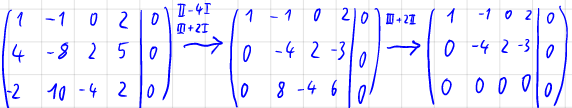
\includegraphics[width=.5\textwidth]{Dateien/00/12BasisKernGauss.PNG}
\end{center}
    \item \textbf{Koeffizienten bestimmen}:\\
    Wir können also $\dim \mathbb{R}^4-\rg A=4-2=2$ Variablen frei wählen.\\
    Seien $c=:r\in\mathbb{R}$ und $d=:t\in\mathbb{R}$. Es folgen die Gleichungen
    \begin{align*}
        -4b+2r-3t=0\Leftrightarrow b&=\frac{1}{2}r-\frac{3}{4}t\\
        a-\underbrace{\BracedIn{\frac{1}{2}r-\frac{3}{4}t}}_b+2t\Leftrightarrow a&=\frac{1}{2}r-\frac{11}{4}t.
    \end{align*}
    \item \textbf{Lösungsmenge aufschreiben}:\\
    Die Lösungsmenge des Gleichungssystems $F(v)=Av=0$ ist also
    \begin{equation*}
        L=\left\{r'\Matrix{1\\1\\2\\0}+t'\Matrix{-11\\-3\\0\\4}\furdas r',t'\in\mathbb{R}\right\},
    \end{equation*}
    wobei wir, da $r,t$ ja beliebig gewählt waren, diese noch skaliert haben.
    \item \textbf{Basis des Kerns ablesen}:\\
    Somit bilden die Vektoren $b_1=\Matrix{1\\1\\2\\0}$ und $b_2=\Matrix{-11\\-3\\0\\4}$ also eine Basis des Kerns von $F$. wir haben
    \begin{equation*}
        \ker F=\Spann{\Matrix{1\\1\\2\\0},\Matrix{-11\\-3\\0\\4}}.
    \end{equation*}
\end{enumerate}
\textbf{Bild}:\\
Das Bild muss aufgrund der Dimensionsformel\footnote{$\dim\im F=\rg F=\dim\mathbb{R}^4-\dim\ker F=4-2=2$} die Dimension 2 haben.\\
Alternativ können wir auch auf die darst. Matrix schauen und sehen, dass diese $\rg A=\rg F=2=\dim\im F$ hat.\\
Wenn wir uns nun also zwei linear unabhängige Spaltenvektoren aus $A$ schnappen, so bilden diese schon eine Basis von $\im F$, also z. B.
\begin{equation*}
    \im F=\Spann{\Matrix{1\\4\\-2},\Matrix{-1\\-8\\10}}.
\end{equation*}
Alternativ könnten wir die Spaltenvektoren als Zeilenvektoren aufschreiben und wieder Gauß anwenden:
\begin{center}
    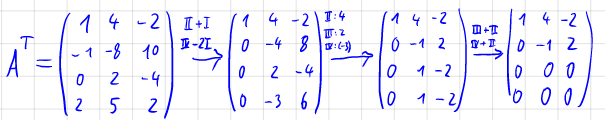
\includegraphics[width=.5\textwidth]{Dateien/00/12BildGauss.PNG}
\end{center}
Die alternative Basis des Bildes können wir nun einfach ablesen:
\begin{equation*}
    \im F=\Spann{\Matrix{1\\4\\-2},\Matrix{0\\-1\\2}}.
\end{equation*}
\end{Beispiel}
\subsubsection{Erneutes Vokabelgewitter}
Abschließend lernt ihr noch ein paar Begrifflichkeiten kennen, die spezielle lineare Abbildungen beschreiben. Diese werden vor allem nächstes Semester wichtig sein.
\begin{Def}
{Dualraum}
\begin{tabular}{c l}
\parbox[b]{10cm}{
Für jeden Vektorraum $V$ über einem Körper $\mathbb{K}$ bezeichnen wir die Menge aller linearen Abbildungen $V\to\mathbb{K}$ als \red{Dualraum $V^*:=L(V,\mathbb{K})$}.
} & 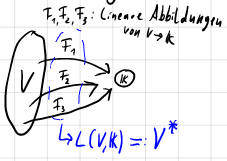
\includegraphics[width=.21\textwidth]{Dateien/00/12Dualraum.PNG}
\end{tabular}
\end{Def}
\begin{Def}
{Endomorphismus}
Lineare Abbildungen aus einem Vektorraum $V$ \underline{in sich selbst}, d. h. $F:V\to V$, nennen wir \red{Endomorphismen}.\\
Diese Menge\footnote{Die ja wieder ein Vektorraum ist, weil wir Linearkombinationen aus solchen Abbildungen bilden können, die wieder Vektoren sind} hat die Bezeichnung $\End(V):=L(V,V)$.\\
\blue{Auf endlichdimensionalen Vektorräumen mit $\dim V=n$ ist die darstellende Matrix dann eine $(n\times n)$-Matrix.}
\end{Def}
Die nächsten beiden Definitionen sind weitere Beispiele für Gruppen, welche wir im letzten Semester definiert hatten.
\begin{Def}{Automorphismus}
Ist ein Endomorphismus bijektiv (d. h. ein Isomorphismus), so nennen wir ihn \red{Automorphismus}.\\
Diese Menge hat die Bezeichnung $(\overbrace{\GL(V)}^{\footnote{Wenn $V$ endlichdimensional ist}}=)\Aut (V)\subseteq \End(V)$
Warum ist dies eine Gruppe?\\
Als Verknüpfung können wir die Komposition von Abbildungen verwenden, die aufgrund der Bijektivität alle erforderlichen Eigenschaften erfüllt. Automorphismen sind invertierbar. Die Identitätsabbildung ist das neutrale Element.\\
Diese Gruppe ist nicht kommutativ.
\end{Def}
\begin{Def}{Allgemeine lineare Gruppe (2/2)}
Ein Spezialfall tritt auf, wenn der Vektorraum $V$ \underline{endlichdimensional} ist.\\
Hier nennen wir Aut($V$) auch \red{GL($V$)}.\footnote{auch \textit{allgemeine lineare Gruppe} (\underline{G}eneral \underline{L}inear Group) genannt.}\\
Betrachte nun $V=\mathbb{K}^n$\footnote{Denn wie wir wissen, sind alle $n$-dimensionalen Vektorräume hierzu isomorph, d. h. es gibt eine bijektive lineare Abbildung zwischen $\mathbb{K}^n$ und diesen Räumen}.\\
In diesem Fall ist die darstellende Matrix der Automorphismen eine $n\times n$-Matrix.\\
Weil Automorphismen bijektiv sind, gilt\\ $\GL(V)=\{A\in\Met(n,\mathbb{K})\furdas \rg A=n\}=\{A\in\Met(n,\mathbb{K})\furdas \ker A=\{0\}\}=\{A\in\Met(n,\mathbb{K})\furdas \det A \neq 0\}$.\\
Es handelt sich also\footnote{bei endlichdimensionalen VR} genau dann um einen Automorphismus, wenn die darstellende Matrix invertierbar ist.
\end{Def}
\begin{Satz}
{Satz}{Vorgriff: Determinante und Isomorphie}
Für $(n\times n)$-Matrizen definieren wir bald die Determinante.\\
Diese gibt u.a. Auskunft darüber, ob der zugehörige Endomorphismus ein Automorphismus ist.\\
Ein Endomorphismus $F$ mit darst. Matrix $A$ ist genau dann auch ein Isomorphismus, wenn $\det(A)\neq 0$ ist.\\
Die Determinante ist eng mit dem Rang einer Matrix verknüpft.
\end{Satz}
\begin{figure}[htbp]
\centering
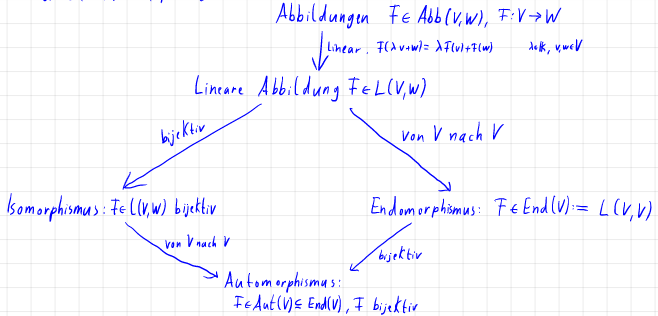
\includegraphics[width=.8\textwidth]{Dateien/00/12UbersichtBegriffe.PNG}
\caption*{Übersicht über die Zusammenhänge zwischen den Begriffen, die wir kennengelernt haben.}
\end{figure}

\subsection[Anhang]{Anhang: Betrachtung der $\phi_B$ und $\phi_{B'}$ aus Bsp. 12.11}\label{sssec:12DarstMatrixlang}
Dieser Anhang ist für alle von euch, die genauer interessiert, was eigentlich hinter den Kulissen abgeht. Meiner (Fabians) Meinung nach ist das nett zu wissen, aber keineswegs unentbehrlich.\\
Wir beziehen uns auf \hyperref[beisp:12DarstMatrix]{Bsp. 12.11}, wo wir ja die darstellende Matrix von $F:\mathbb{R}^2\to\mathbb{R}[x]_{\leq2}=:F:V\to W$ finden wollten.\\
Dort hatten wir 
\begin{equation*}
    F:\mathbb{R}^2\to \mathbb{R}[x]_{\leq 2},\,F(a,b)=a+(a-b)x+5bx^2\quad (\text{z. B. } F(1,2)=1-x+10x^2).
\end{equation*}
Wie sehen nun die Abbildungen $\phi_B$ und $\phi_{B'}$ aus der Definition der darst. Matrix aus?\\
Diese sollen nun Abbildungen aus $\mathbb{R}^2\to V$ bzw. $\mathbb{R}^3\to W$ sein, sodass die kanonischen Einheitsvektoren von $\mathbb{R}^2$ bzw. $\mathbb{R}^3$ auf $B$ bzw. $B'$ abgebildet werden.
\begin{itemize}
    \item Für $\phi_B:\mathbb{R}^2\to V$ haben wir:\\
    $\phi_B(e_j)\overset{!}{=}b_j$. Die kanonische Matrix dieser Abbildung ist:
    \begin{equation*}
        A_{\phi_B}=\Matrix{1&-1\\1&1},\text{ denn } A_{\phi_B}e_1=\Matrix{1\\1}=b_1\text{ und } A_{\phi_B}e_2=\Matrix{-1\\1}=b_2.\,\checkmark
    \end{equation*}
    \item Analog haben wir für $\phi_{B'}:\mathbb{R}^3\to W$
    \begin{equation*}
        A_{\phi_{B'}}=\Matrix{1&0&0\\2&0&-1\\0&3&0}, \text{ denn } A_{\phi_{B'}}e_1=\Matrix{1\\2\\0}\overset{\wedge}{=}1+2x=b_1,\text{ Rest analog}.\,\checkmark
    \end{equation*}
    \item Für die Anwendung benötigen wir nun die Umkehrabbildung $\phi_{B'}^{-1}:W\to\mathbb{R}^3$:
    \begin{equation*}
        A_{\phi_{B'}}^{-1}=\Matrix{1&0&0\\0&0&1/3\\2&-1&0}.
    \end{equation*}
    \blue{\textbf{Anmerkung}: Das Werkzeug zum Invertieren von Matrizen erhaltet ihr im zweiten Semester. Keine Angst, das müsst ihr aktuell nicht können.}
    \item Damit ist die darstellende Matrix in ihren einzelnen Komponenten also
    \begin{align*}
        j=1:&\quad A e_1=\phi_{B'}^{-1}(F(\phi_B(e_1)))=\phi_{B'}^{-1}(F(1,1))=\Matrix{1&0&0\\0&0&1/3\\2&-1&0}\Matrix{1\\0\\5}=\Matrix{1\\5/3\\2}\\
        j=2:&\quad A e_2=\phi_{B'}^{-1}(F(\phi_B(e_2)))=\phi_{B'}^{-1}(F(-1,1))=\Matrix{1&0&0\\0&0&1/3\\2&-1&0}\Matrix{-1\\-2\\5}=\Matrix{-1\\5/3\\0}.
    \end{align*}
    \item Also ist $M_B^{B'}(F)$ (wie schon oben herausgefunden) einfach
    \begin{equation*}
        M_B^{B'}(F)=\Matrix{1&-1\\5/3&5/3\\2&0}.
    \end{equation*}
\end{itemize}


\subsection{Äquivalenzrelationen und Orientierung}
\blue{Bevor wir uns dem nächsten großen Thema, den \red{Eigenvektoren}, widmen, folgt nun ein kurzer Überblick über das Konzept der Äquivalenzrelationen, den Quotientenraum und die Orientierung von Basen.}
\begin{Wiederholung}
{Relation}
Eine \red{Relation} $R$ auf einer Menge $X$ kann als Teilmenge von $X\times X$ aufgefasst werden.\\
Diese Teilmenge umfasst dann alle Paare $(x,y)\in X\times X$, für die die Relation erfüllt ist.
\end{Wiederholung}
Bereits bekannte Relationen sind die \red{Ordnungsrelationen} ($>,<,\leq,\geq,=$), aber wir können natürlich auch jegliche andere Paare definieren, z.B. die Relation $\hat{R}_2$ auf $\mathbb{N}$, die alle natürlichen Zahlen verknüpft, die das durch den Faktor 2 verbunden werden, d.h.\\
$\hat{R}_2:=\Menge{(x,y)\in\mathbb{N}^2}{x=2y\lor y=2x}$.\\
Von diesen allgemeinen Relationen betrachten wir nun einen Spezialfall:
\begin{Def}
{Äquivalenzrelation}
Wir nennen eine Relation $\sim$ auf einer Menge $X$ eine \red{Äquivalenzrelation}, wenn sie folgende drei Eigenschaften erfüllt:\\
\begin{tabularx}{\linewidth}{p{2.2cm}|X|X}
    \textbf{Name} &\textbf{Forderung}&\textbf{Erklärung} \\
    \hline
    \blue{Reflexivität:} & $x\sim x\,\forall x\in X$ & $x$ ist zu sich selbst äquivalent.\\
    \hline
    \blue{Symmetrie:} & $x\sim y\implies y\sim x\,\forall x,y\in X$ & Ist $y$ zu $x$ äquivalent, so ist auch $x$ zu $y$ äquivalent.\\
    \hline
    \blue{Transitivität:}  & $x\sim y\land y\sim z\implies x\sim z\,\forall x,y,z\in X$ & Sind $x$ und $y$ und zudem $y$ und $z$ äquivalent, so sind auch $x$ und $z$ äquivalent.
\end{tabularx}
\end{Def}
\begin{Def}
{Äquivalenzklasse}
Gemeinsam mit der Äquivalenzrelation $\sim$ definiert jedes Element aus $X$ dann eine \red{Äquivalenzklasse $[x]$}:
\begin{equation}
    [x]:=\Menge{y\in X}{y\sim x},
\end{equation}
diese beinhaltet also alle Elemente aus $X$, die zu $x$ äquivalent sind.\\
Als $X/\sim$ bezeichnen wir die Menge aller möglichen Äquivalenzklassen.
\end{Def}
\begin{Beispiel}
{Geburtsjahräquivalenz (1/3)}
Für die Menge aller Studierenden an der Physikfakultät ist \textit{das gleiche Geburtsjahr haben} eine Äquivalenzrelation. Die Menge aller möglichen Äquivalenzklassen würde in diesem Fall alle vertretenen Geburtsjahre beinhalten.\\
Andere Äquivalenzrelationen wären der Geburtsort oder andere eindeutige Eigenschaften der Studierenden.
\end{Beispiel}
\begin{Beispiel}
{Restklassen (2/3)}
Wir betrachten die Menge $X=\mathbb{Z}$ der ganzen Zahlen und eine natürliche Zahl $n>1$.\\
Durch 
\begin{equation*}
    x\sim y\iff n\tx{ teilt }(x-y)
\end{equation*}
wird dann eine Äquivalenzrelation auf $\mathbb{Z}$ definiert.\footnote{Als Beispiel sei $n=3$ genannt. In diesem Fall sind 5 und 8 äquivalent, 5 und 9 aber nicht.} Zwei ganze Zahlen sind hier also genau dann äquivalent, wenn sie bei Division durch $n$ den selben Rest lassen.\\
Mit $\mathbb{Z}/n\mathbb{Z}$ oder einfach $\mathbb{Z}_n$ bezeichnet man die Menge der \red{Restklassen}, also die Klassen, die durch den Rest bei Division durch $n$ definiert sind.\\
Diese Klassen kann man durch
\begin{equation*}
    [x]+[y]:=[x+y]\quad \tx{und}\quad [x]\cdot [y]:=[x\cdot y]
\end{equation*}
mit einer Addition und Multiplikation versehen, sodass $(\mathbb{Z}_n,+)$ eine kommutative Gruppe mit neutralem Element $[0]$\footnote{also die Äquivalenzklasse, die alle Zahlen enthält, die durch $n$ ohne Rest teilbar sind} ist.\\
Falls $p$ eine Primzahl ist, ist $(\mathbb{Z}_p,+,\cdot)$ sogar ein Körper (mit dem neutralen Element der Multiplikation $[1]$).
\end{Beispiel}
\begin{Beispiel}
{Die Betragsäquivalenz}
\begin{wrapfigure}{r}[0pt]{.25\textwidth}
 \vspace{-15pt}
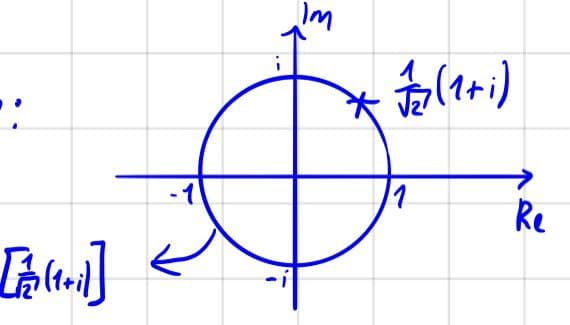
\includegraphics[width=.25\textwidth]{Dateien/01/01Betragsklassen.jpg}
 \vspace{-15pt}
\end{wrapfigure}
Auf den komplexen Zahlen sei $x\sim y\iff \Abs{x}=\Abs{y}$ mit $x,y\in\mathbb{C}$.\\
Dies ist eine Äquivalenzrelation, denn die Reflexivität ist klar, die Symmetrie folgt aus der Symmetrie des Betrages und die Transitivität folgt aus der Transitivität der Gleichheit.\\
Äquivalenzklassen sind dann Kreise in der komplexen Ebene, im Bild seht ihr die Äquivalenzklasse $[\frac{1}{\sqrt{2}}(1+i)]$.\\
Die Menge aller Äquivalenzklassen $\mathbb{C}\,\setminus\sim$ entspricht dann z.B. allen positiven reellen Zahlen, da diese jeweils einzigartige Äquivalenzklassen definieren.
\end{Beispiel}
Das Konzept der Äquivalenzklassen nutzen wir nun, um Äquivalenz zwischen Vektoren in Bezug auf einen Untervektorraum herzustellen:
\begin{Def}
{Quotientenraum}
Für Unterräume $U\subseteq V$ eines Vektorraums $V$ über einem Körper $\mathbb{K}$ können wir (auf $V$!) eine Äquivalenzrelation für Vektoren $v,w\in V$ definieren:
\begin{equation}
    v\sim w\iff v-w=u\in U.
\end{equation}
Die Menge $V/U=\Menge{[v]}{v\in V}$ aller Äquivalenzklassen\footnote{z.B. die zu $U$ parallelen Geraden, siehe im folgenden Beispiel} nennen wir auch \red{Quotientenraum} oder \red{Quotientenvektorraum}\footnote{Siehe auch unter \href{https://de.wikipedia.org/wiki/Faktorraum}{Wikipedia}.} von $U$.
\end{Def}
Was bedeutet diese Relation anschaulich?\\
Wir klassifizieren Vektoren $v,w\in V$ als gleich, sobald ihre Differenz im Unterraum $U$ liegt. Umgeschrieben können wir $w=u+v$ schreiben, $v$ und $w$ sind also äquivalent, wenn man durch Verschiebung von $v$ um einen Vektor aus $U$ den Vektor $w$ erzeugen kann. Dies wird vielleicht mit einem Beispiel verständlicher:
\begin{Beispiel}
{Quotientenraum im $\mathbb{R}^2$}
\begin{wrapfigure}{r}[0pt]{.35\textwidth}
 \vspace{-15pt}
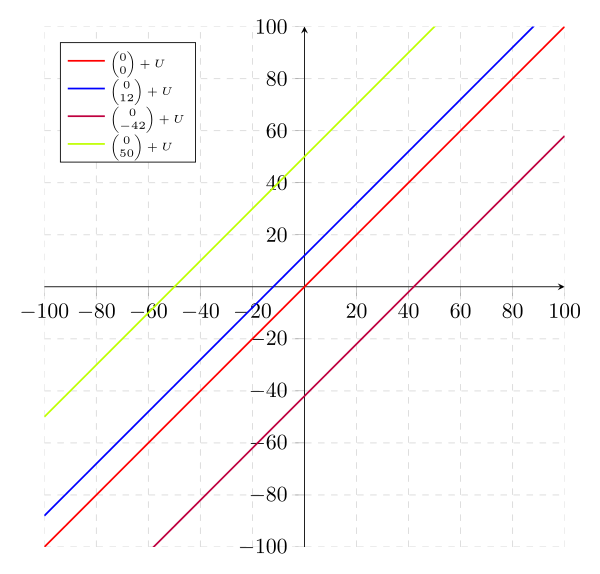
\includegraphics[width=.35\textwidth]{Dateien/01/01Quotientenraum.png}
\end{wrapfigure}
Sei $V=\mathbb{R}^2$ und $U$ eine Gerade mit\\
$U=\Menge{v\in V}{v=\MatrixInline{1\\1}x,\, x\in \mathbb{R}}$.\\
Dann sind mit $\sim$ alle Punkte, die jeweils auf einer Geraden parallel zu $U$ liegen zueinander äquivalent und wir können für die Äquivalenzklassen eines Vektors $v$ auch schreiben
\begin{equation*}
    [v]=\Menge{w\in V}{w=v+u,\,u\in U}.
\end{equation*}
Dies ist im nebenstehenden Bild (von Wikipedia) illustriert.
\end{Beispiel}



\Tipps{2}{
\begin{enumerate}
\item Orientiert euch an unseren Beispielen zur Basisfindung im Kapitel zu Vektorräumen.
\item Hierzu haben wir z. B. Beispiel \ref{beisp:basisbildkern} angesehen.
\item Schlagt hier die genauen Definitionen der Linearität und der Matrixmultiplikation nach, dann dürfte das nicht sonderlich umfangreich sein. Für c) könnte b) vielleicht nützlich sein.
\item Schaut bei Problemen gern die Hilfestellungen und Beispiele zu Äquivalenzrelationen an. Hier müsst ihr einfach stumpf die Eigenschaften überprüfen oder euch überlegen, weshalb eine davon nicht klappt.
\end{enumerate}
}